\documentclass[letterpaper,twoside,12pt]{article}
\usepackage[dvips]{graphicx}
\usepackage[margin=0.8in]{geometry}
\usepackage{caption}
\usepackage{amsmath}
\usepackage{amssymb}
\usepackage[T1]{fontenc}
\usepackage{natbib}
\usepackage{authblk}
\bibliographystyle{agu08}

\newcommand{\ud}{\mathrm d}
\newcommand{\uj}{\mathrm{j}}
\newcommand{\bz}{\mathbf{z}}
\newcommand{\Real}{\mathrm{Re}}
\newcommand{\Imag}{\mathrm{Im}}
\newcommand{\dif}{\mathrm{d}}
\newcommand{\sigsig}{\sigma_1\sigma_2}
\newcommand{\varss}{\varsigma_1\varsigma_2}
\newcommand{\hvarss}{\hat{\varsigma}_1 \hat{\varsigma}_2}


\title{Normality Test for 2-bit Stream Data in Mark-5 Files}

\author[1]{L. V. Benkevitch}
\affil[1]{\small MIT Haystack observatory, Westford, MA 01886, USA.}


\begin{document}

\maketitle

\begin{abstract}
The radio astronomy data from a single dish are recorded in M5B (Mark-5) or VDIF formatted files. The recorded data are supposed to be Gaussian white noise. A corrupted data segment can be spotted at the output of correlation stage. However, the correlation is expensive and vastly increases the bulk of data to be analyzed for spurious parts. Here we consider a problem of finding non~Gaussian (or non-normal) single-dish data segments in M5B files.

The problem may be thought about from a security standpoint. Suppose someone (a malicious character) wishes to hack a system and figures an approach would be to embed some malicious code in. Is it possible to detect the embedded (non-Gaussian) data within a frame or multiple frames before the correlator? Also, even though an algorithm can be determined, is it possible to make its implementation fast enough? The data files are large (up to a hundred gigabytes).

Our solution is based on Pearson's $\chi^2$ test. The null hypothesis states that the data in file  are consistent with the normal distribution. If the data in a part of the file do not pass the test at the significance level 0.05, the null hypothesis is rejected, and the data fragment is flagged.

The algorithm runs on the GPU (Graphics Processing Unit), which provides high speed computations.
\end{abstract}


\section{Quantization and M5B Data Structure}

The analog signal from a single antenna/dish is supposed to be Gaussian noise $N(\mu,\sigma)$ with the expectation $\mu$ and standard deviation (rms) $\sigma$ distributed according to the normal law with the probability density function (PDF):

\begin{equation}
  \label{normal_pdf}
  N(\mu,\sigma) =  \frac{1}{\sigma\sqrt{2\pi}} e^{-\frac{(x-\mu)^2}{2\sigma^2}}.
\end{equation}

The signal is centered to ensure zero $\mu$ and its band is filtered into 16 frequency channels each of which is passed through the 4-level quantizer with the characteristic shown in Fig.~\ref{quant4lvl}.  The quantizer has just three switching thresholds, $-\theta$, 0, and $\theta$, so it is characterized with the only parameter, the adjustable quantization threshold $\pm\theta$. Note that the hardware deals with voltage thresholds, $\pm v_0$, but $\theta$ is expressed in the signal STDs, thus it is dimensionless, $\theta = v_0/\sigma$. The quantizer output only takes four values as in Tab.~\ref{quant_io}. These values are saved in the M5B file.


\begin{figure}[h!]
  \begin{center}
  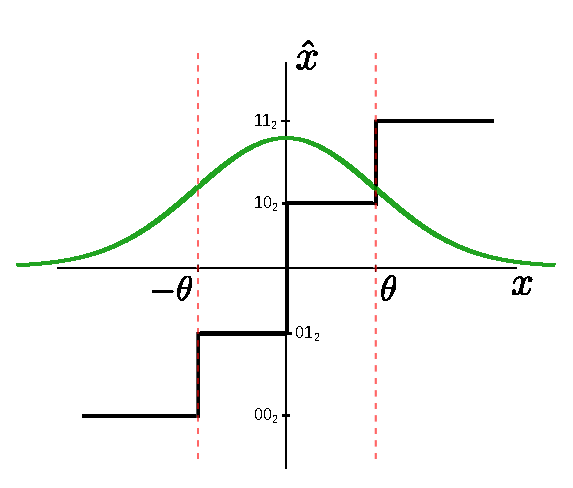
\includegraphics[width=25pc]{fig_4_Level_Quantization_Pattern_impr.eps}
  %\noindent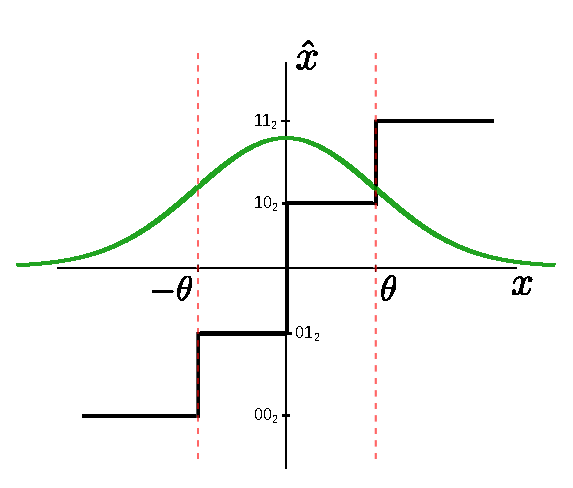
\includegraphics[width=20pc]{fig_4_Level_Quantization_Pattern_impr.eps}
  %\includegraphics[width=\linewidth]{}
  \caption{4-level quantization.}
  \label{quant4lvl}
  \end{center}
\end{figure}


\begin{table}[h!]
  \begin{center}
    \caption{Quantizer}
    \label{quant_io}
    \begin{tabular}{c|c}
      \textbf{Input} & \textbf{Output} \\
      \hline
      $-\infty$ to $-\theta$ & 0 \\
      $-\theta$ to 0         & 1 \\
      0 to $\theta$          & 2 \\
      $\theta$ to $+\infty$  & 3 \\
    \end{tabular}
  \end{center}
\end{table}


The M5B file can be considered as an array of 10016-byte frames. Each frame consists of 2504 32-bit words (\verb@unsigned int@ or  \verb@uint@ in C/C++). The first 4 words comprise the frame header, so a frame has 2500 words of pure data. Each 32-bit data word is subdivided into 16 2-bit channels, numbered from 0 to 15. The header contains the sync word \verb@0xdec0de5c@, 23-bit long frame number within second (reset to zero each new second), one flag bit to tag the frame invalid, 8-bit long channel ID, BCD Time Code Word 1 (‘JJJSSSSS’), BCD Time Code Word 2 (‘.SSSS’), and  16-bit CRCC.

Unfortunately, the header does \emph{not} contain the quantization threshold value $\theta = v_0/\sigma$, which is necessary for the statistical testing. In order to estimate $\theta$, the algorithm has to spend precious time on its linear search as will be described further. 




\section{Statistical Testing Data Normality Using $\chi^2$}

We need to test if the data in each of the 16 channels are sampled from a normally distributed population (the null hypothesis) or not (the alternative hypothesis). In each frame and channel, there are $N=$ 2500 data samples divided into $n=4$ categories by their values, 0, 1, 2, and 3. The counts of data samples in each category form the 4 histogram bins $B_i, i=\overline{0 .. 3}$, so $\sum_{i=0}^3 B_i = N$. The Pearson's $\chi^2$ test is based on comparing the observed data counts with the expected (theoretical) counts $E_i, i=\overline{0 .. 3}$ obtained from the normal PDF~\eqref{normal_pdf} as $E_i = Np_i$. Here $p_i$ is the probability that a random value sampled from $N(0,\sigma)$ is within the $i$-th interval. The intervals are given in Tab.~\ref{quant_io}, where $i$ is an Output value. 

For each data frame the value of the test-statistic is calculated as 

\begin{equation}
  \label{chi2_calc}
  X^2 = \sum_{i=0}^3 \frac{(B_i - E_i)^2}{E_i}.
\end{equation}


The $X^2$ test-statistic asymptotically approaches the $\chi^2_{k=3}$ distribution, where $k = n - 1 = 3$ is the number of degrees of freedom. The $\chi^2_{k=3}$ PDF is shown in Fig.~\ref{chi2_pdf}. The statistic $X^2$ is a random value showing how close are the observation frequencies $B_i$ to the perfect, theoretical frequencies $E_i$. The $\chi^2_{k=3}$ PDF has maximum at $X^2=1$ and the mean at $X^2=k=3$. This means that if $X^2$ is distributed as $\chi^2_{k=3}$ its most probable random values will be concentrated somewhere around the mean 3 and not much further. But how much further? The area under the $\chi^2_{k=3}$ PDF curve in Fig.~\ref{chi2_pdf} over an interval $[a,b]$ equals to the probability that the random value will appear within this interval. If we want to be 95\% confident that the data is distributed normally, $X^2$ cannot exceed the critical value $\chi^2_{cr}$ such that the probability for $X^2$ to appear within the interval $[0 .. \chi^2_{cr}]$ is $p=0.95$. The critical $\chi^2_{k=3}$ value can be calculated as the value of $\chi^2$ Probability Point Function or PPF, the inverse of the Cumulative Distribution Function or CDF. In Python this is done as $\verb@scipy.stats.chi2.ppf(1-alpha, k)@$, where $\alpha = 0.05$ is the level of significance. In our case $\chi^2_{cr} = 7.81$. 

Thus, our algorithm flags a channel data in frame as non-Gaussian if its $X^2 > 7.81$, the probability of incorrectly rejecting the null hypothesis being $\alpha = 0.05$. 

\begin{figure}[h!]
  \begin{center}
  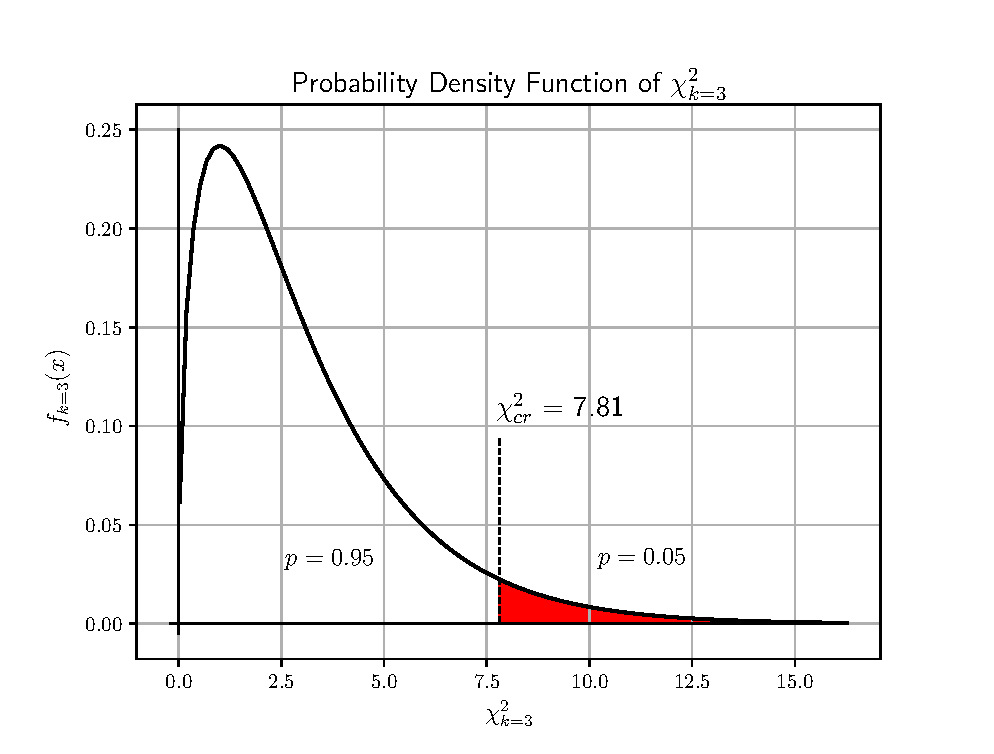
\includegraphics[width=25pc]{fig_chi2_pdf.eps}
  %\noindent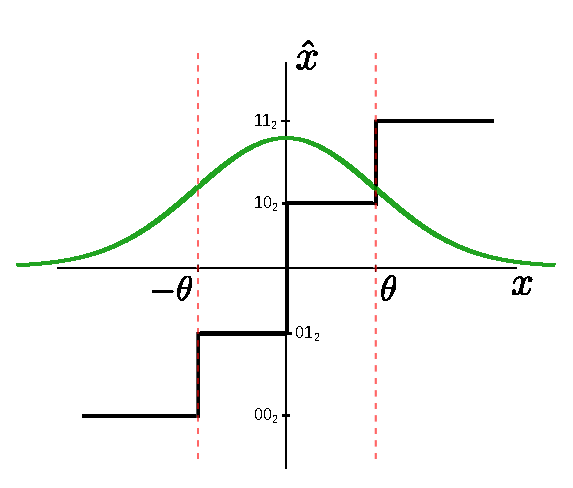
\includegraphics[width=20pc]{fig_4_Level_Quantization_Pattern_impr.eps}
  %\includegraphics[width=\linewidth]{}
  \caption{Chi-squared distribution function.}
  \label{chi2_pdf}
  \end{center}
\end{figure}



\section{Estimation of Quantization Threshold Using Linear Search}



\end{document}



